\chapter{Results and Evaluation}
In this chapter we are going to show the best results obtained by setting up the training phase as described in the previous chapters. Most of the parameter tuning was done on just one dataset\footnote{The Reuters Corpus, RCV1}, and then the same setup was used to produce results for all our datasets.
\section{Metrics used}

\section{Results for single topic authorship attribution}
\subsection{Reuters Corpus results}

\begin{table}[h!]
	\begin{center}  
		\caption[Reuters Corpus Results - 10 authors]{Accuracy score and F1 macro score for Reuters Corpus 10 authors CCAT category.} 
		\label{tab:tableRCV1_10}
		%\resizebox{\linewidth}{!}{  %
		\begin{tabular}{| p{5 cm} | c | c |}
			\hline 
			Model & Accuracy & F1 macro \\
			\hline
			LinearSVC (combinedDFs), tfidf, simple tokenizer & 0.878 & 0.876 \\ \hline
			LinearSVC (combinedDFs), tfidf, only-remove-quotes-tokenizer & 0.908 & 0.906 \\ \hline
			LinearSVC (combinedDFs), tfidf, only-remove-quotes-tokenizer (threshold 1),
			ngram=(1,2) & 0.922 & 0.921 \\ \hline
			%\bottomrule 
		\end{tabular} 
		%}
	\end{center}
\end{table}

\begin{table}[h!]
	\begin{center}  
		\caption[Reuters Corpus Results - 50 authors]{Accuracy score and F1 macro score for Reuters Corpus 50 authors CCAT category.} 
		\label{tab:tableRCV1_50}
		%\resizebox{\linewidth}{!}{  %
		\begin{tabular}{| p{5 cm} | c | c |}
			\hline 
			Model & Accuracy & F1 macro \\
			\hline
			LinearSVC (combinedDFs), tfidf, stock tokenizer & 0.7644 & 0.76 \\ \hline
			LinearSVC (combinedDFs), tfidf, only-remove-quotes-tokenizer & 0.7884 & 0.7842 \\ \hline
			LinearSVC (combinedDFs), tfidf, only-remove-quotes-tokenizer (threshold 1),
			ngram=(1,2) & 0.7984 & 0.7949 \\ \hline
			%\bottomrule 
		\end{tabular} 
		%}
	\end{center}
\end{table}


\begin{table}[h!]
	\begin{center}  
		\caption[Reuters Corpus Benchmark - 10 and 50 authors]{Accuracy score for Reuters Corpus 10 and 50 authors in the CCAT category.} 
		\label{tab:tableRCV1_10_benchmark}
		%\resizebox{\linewidth}{!}{  %
		\begin{tabular}{| p{5 cm} | c | c |}
			\hline 
			Model & RCV1-10 & RCV1-50 \\
			\hline
			D2V words & 0.8280 & 0.7524 \\ \hline
			Local histograms & 0.8640 & - \\ \hline
			Tensor space models & 0.8080 & - \\ \hline
			Character and word n-grams & 0.7940 & - \\ \hline
			N-gram feature selection & - & 0.7404 \\ \hline
			N-gram feature selection & - & 0.7404 \\ \hline
			\textbf{Our approach} & \textbf{0.9220} & \textbf{0.7984} \\ \hline
			%\bottomrule 
		\end{tabular} 
		%}
	\end{center}
\end{table}


\subsection{GDELT Corpus results}

\begin{table}[h!]
	\begin{center}  
		\caption[GDELT Results - 45 authors]{Accuracy score and F1 macro score for GDELT 45 authors.} 
		\label{tab:tableGDELT}
		%\resizebox{\linewidth}{!}{  %
		\begin{tabular}{| p{5 cm} | c | c |}
			\hline 
			Model & Accuracy & F1 macro \\
			\hline
			LinearSVC (combinedDFs), tfidf, stock tokenizer & 0.7355 & 0.7090 \\ \hline
			LinearSVC (combinedDFs), tfidf, only-remove-quotes-tokenizer & 0.7426 & 0.7173 \\ \hline
			LinearSVC (combinedDFs), d2v dmm & 0.7716 & 0.7489 \\ \hline
			%\bottomrule 
		\end{tabular} 
		%}
	\end{center}
\end{table}


\subsection{Amazon Food Reviews Corpus results}

\begin{table}[h!]
	\begin{center}  
		\caption[Amazon Food Reviews Results - 50 authors]{Accuracy score and F1 macro score for Amazon Food Reviews 50 authors dataset.} 
		\label{tab:tableAFR}
		%\resizebox{\linewidth}{!}{  %
		\begin{tabular}{| p{5 cm} | c | c |}
			\hline 
			Model & Accuracy & F1 macro \\
			\hline
			LinearSVC (combinedDFs), tfidf, simple tokenizer & 0.7704 & 0.7674 \\ \hline
			LinearSVC (combinedDFs), tfidf, stock tokenizer & 0.7836 & 0.7817 \\ \hline
			LinearSVC (combinedDFs), tfidf, only-remove-quotes-tokenizer,
			ngram=(1,2) & 0.8388 & 0.8368 \\ \hline
			%\bottomrule 
		\end{tabular} 
		%}
	\end{center}
\end{table}

\section{The Guardian Corpus results}

\begin{table}[h!]
	\begin{center}  
		\caption[The Guardian Corpus Results]{Accuracy score and F1 macro score for The Guardian Corpus with LinearSVC (combinedDFs), tfidf, only-remove-quotes-tokenizer.} 
		\label{tab:tableTGC}
		%\resizebox{\linewidth}{!}{  %
		\begin{tabular}{| p{5 cm} | c | c |}
			\hline 
			Training topic vs Test topic & Accuracy & F1 macro \\
			\hline
			Politics vs Books & 0.7446 & 0.7640 \\ \hline
			Politics vs World & 0.7560 & 0.7470 \\ \hline
			Politics vs Uk & 0.7890 & 0.7010 \\ \hline
			Politics vs Society & 0.8863 & 0.7430 \\ \hline
			\textbf{Average} & \textbf{0.7940} & \textbf{0.7388} \\ \hline
			%\bottomrule 
		\end{tabular} 
		%}
	\end{center}
\end{table}


\begin{figure}[ht]
	\centering
	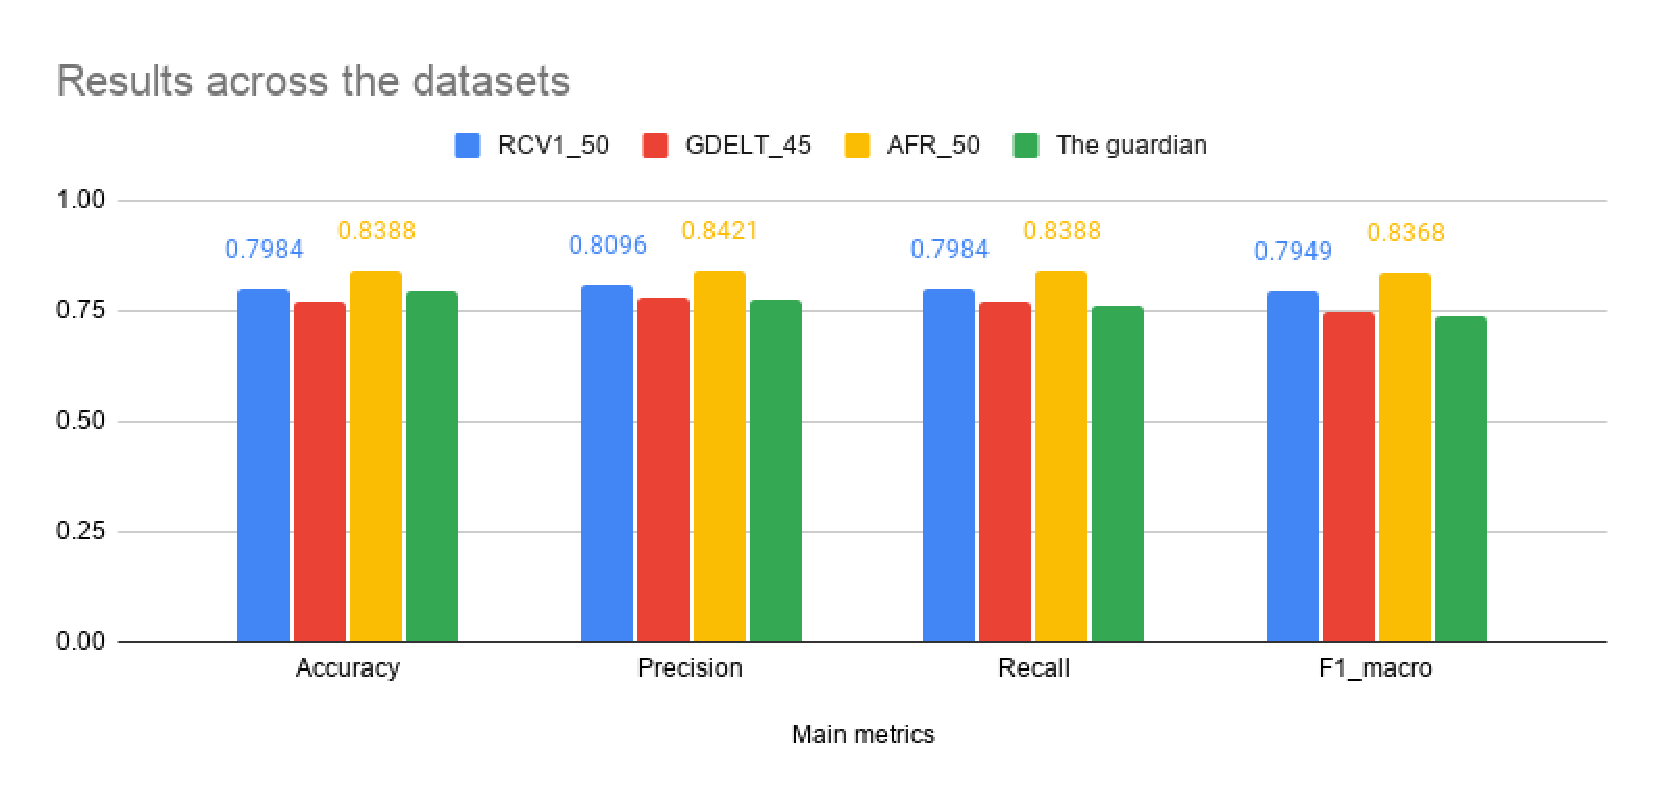
\includegraphics[width=0.8\textwidth, height=1.0\textheight, keepaspectratio]{Results_across_datasets}
	\caption[Best performance across all datasets]{Accuracy, precision, recall and f1-macro for every dataset showing only the best result achieved for each one.}
	\label{fig:results_across_datasets}
\end{figure}
